\section{CEK Machines and Heaps}  

Zombie works on a purely functional language with products, sum types,
and first-class functions called $\lambda_Z$. For simplicity, we treat
the language as untyped in this paper. The syntax of $\lambda_Z$ is
shown in \Cref{fig:syntax}; its semantics are standard. Additional
features supported by the full Zombie implementation, such as
primitive types and input/output, are not relevant to recomputation
and are described in \Cref{sec:impl}.

Importantly, $\lambda_Z$ is purely functional, meaning programs are
totally deterministic: evaluating a given expression in a given
environment always returns the same result. This is essential for
Zombie to work correctly.

\subsection{CEK Machine}

\newcommand{\mytableshape}{p{6em} p{2em} p{1em} p{0.5\textwidth}}
\begin{figure}
\begin{tabular}{\mytableshape}
  Name & $x$ & $::=$ & A set $N$ of distinct names \\
  Expression & $C$ & $::=$ & \(
  x \mid
  \sLet~x=A~\sIn~B \mid
  \lambda x,~A \mid
  F(A) \mid
  (A, B) \mid
  A.0 \mid
  B.1 \mid
  \sLeft~A \mid
  \sRight~B \mid
  \sCase~A~\sOf~\{~\sLeft~x\Rightarrow
        L~|~\sRight~y\Rightarrow R~\} \)
\end{tabular}
\caption{The syntax of $\lambda_Z$. Lower case letters
  represent variables and upper-case letters represent
  expressions. The semantics of each expression is standard.}
\label{fig:syntax}
\end{figure}

\begin{figure}
\begin{tabular}{\mytableshape}
  Environment & $\Env$ & ::= & $[(N, V)]$ \\

  Value & $V$ & $::=$ & $
  \Clos~\Env~N~C \mid
  \VProd~V~V \mid
  \VLeft~V \mid
  \VRight~V $ \\

  Continuation & $K$ & $::=$ & $
  \Done \mid
  \KLookup~K~ \mid
  \KLet~N~\Env~C~K \mid
  \KApp_0~\Env~C~K \mid
  \KApp_1~\Env~N~C~K \mid
  \KProd_0~\Env~C~K \mid
  \KProd_1~V~K \mid
  \KZro~K \mid
  \KFst~K \mid
  \KLeft~K \mid
  \KRight~K \mid
  \KCase~\Env~N~C~N~C~K $ \\
  
  State & & ::= & $\Eval~E~\Env~K \mid \Apply~K~V $ \\
\end{tabular}
\caption{Definitions of values, environments, and states for
  the CEK machine. Note that $E$ represents environments,
  and $C$ represents expressions. Kontinuations $K$ represent
  computation steps that can be applied to a value and are
  named after the corresponding expression type.}
\label{fig:defs}
\end{figure}

The key insight of Zombie is to assign a unique identifier to any
value ever allocated during the program's execution. Conceptually, it
identifies each value with the execution step that allocated it. It
does this using a variant of the CEK machine.

The CEK machine is a well-known abstract machine for executing untyped
lambda calculi, where the machine state consists of three parts:

\begin{enumerate}
  \item \textcolor{blue}{C}ontrol, the expression currently being evaluated.
  \item \textcolor{blue}{E}nvironment,
          a map from the free variables of the Control to their values.
  \item \textcolor{blue}{K}ontinuation, which is to be invoked
          with the value the Control evaluates to.
\end{enumerate}

In this work, it is convenient to split the evaluation phase from the
invocation of the continuation, resulting in a variation of the CEK
machine with the following machine state:
\[
\text{State} \operatorname{::=} \Eval~C~\Env~K \mid \Apply~K~V
\]
The $\Eval$ state stores the classic control-environment-kontinuation,
while $\Apply$ stores a kontinuation and the value to which it is
being applied. The precise syntax of values and kontinuations are
given in \Cref{fig:defs}; their semantics is standard.

Execution in the CEK machine involves a series of transitions between
these machine states; in other words, it is a transition system. To
run a program $C$ in the CEK machine, one creates the initial state
$(\Eval~C~\{\}~\Done)$, with its Control set to the expression to
evaluate, Environment empty, and Kontinuation set to a special $\Done$
kontinuation. The rules of the CEK machine are then used to transition
from one machine state to another, until finally reaching the state
$\Apply~\Done~V$. In that state, $V$ is the result of evaluating
$C$.%
\footnote{Note that, because $\lambda_Z$ is untyped, it contains
non-terminating programs using, for example, the $Y$ combinator. In
the CEK machine, these programs create an infinite sequence of machine
states that do not include a terminating $\Apply~\Done~V$.}
The full CEK transition relation,
  for our variant of the CEK machine,
  is given in \Cref{adx:cek}.

For example, to evaluate a function application $F(X)$
  and apply the kontinuation $K$ to the result,
  the CEK machine first evaluates the function argument:
\begin{mathpar}
  \inferrule{ }{\Eval(F(X), \Env, K) \leadsto \Eval(F, \Env, \KApp_0~K~X)}
\end{mathpar}
Note that the argument $X$ is stored in the $\KApp_1$ kontinuation,
to be evaluated at a later point. The $\KApp_0$ kontinuation basically
represents the one-hole context $\lambda v, v(X)$.

Eventually, assuming the program is well-typed, $F$ will be evaluated
to a closure value ($\Clos$), at which point the CEK machine will
transition to an $\Apply$ state, which will then transition to
evaluating the argument:
\begin{mathpar}
  \inferrule{ }{\Apply(\KApp_0~\Env~X~K, \Clos~\Env'~N~C) \leadsto \Eval(X, \Env, \KApp_1~\Env'~N~C~K)}
\end{mathpar}
Note that the components $\Env'$, $N$, and $C$ of the closure are now
stored in the $\KApp_1$ kontinuation, which basically represents
the one-hole context $\lambda v, (\Clos~\Env'~N~C)(v)$.

Finally, when the argument $X$ has been evaluated to an argument,
  the closure is called:
\begin{mathpar}
  \inferrule{ }{\Apply(\KApp_1~\Env~N~C~K, V) \leadsto \Eval(C, \Env[N=V], K)}
\end{mathpar}
Note that the kontinuation $K$ here refers to the original receiver
  of the value of $F(X)$, which has been carefully passed
  through a series of transition steps.
In other words, during the execution of a program,
  the kontinuation $K$ forms a kind of singly-linked list
  representing the stack of one-hole program contexts
  that evaluation is proceeding within.

A notable property of the CEK machine is that each transition performs
a bounded amount of work. Contrast this to a traditional operation
semantics, where the semantics of a \sCase statement might include a
rule like:

\begin{mathpar}
 \inferrule{
   \Gamma \vdash e \to \Gamma' \vdash e'
 }{\Gamma \vdash
   \sCase~e~\sOf~\{~\sLeft~x\Rightarrow L~|~\sRight~y\Rightarrow R~\}
   \to
   \Gamma' \vdash
   \sCase~e'~\sOf~\{~\sLeft~x\Rightarrow L~|~\sRight~y\Rightarrow R~\}
 }
\end{mathpar}

In such a small-step semantics, derivations form a tree,
  and the antecedent of the inference rule might require
  an arbitrarily-large derivation,
  and thus an arbitrary amount of computation.
In the CEK machine, no such steps exist,
  and derivations in the CEK machine form a flat list.
This property of the CEK machine
  is illustrated graphically in \Cref{fig:constant}.

\begin{figure}
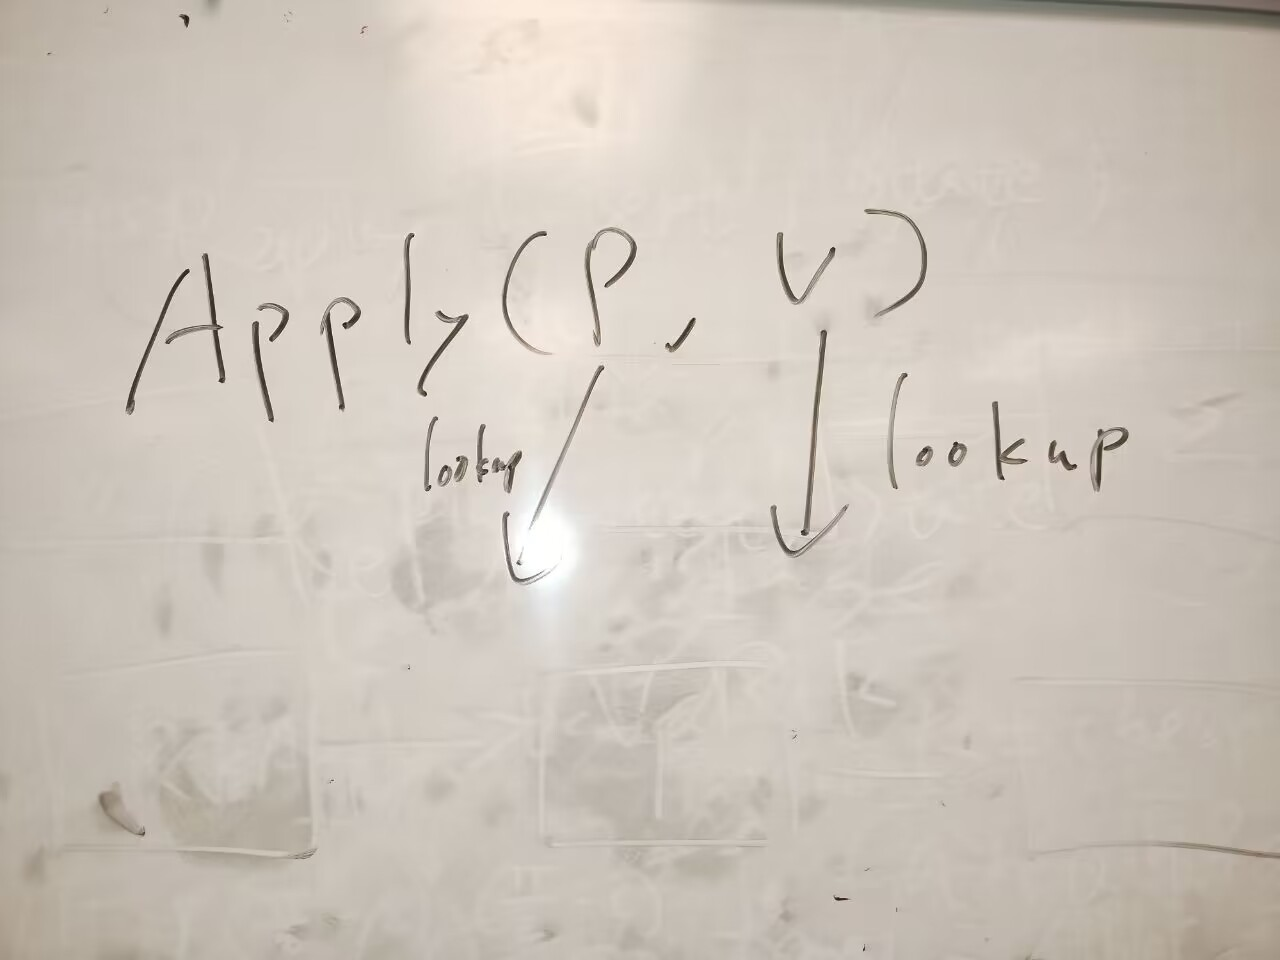
\includegraphics[width=0.5\columnwidth]{img1}
\caption{
  Unlike a traditional small-step or big-step operational semantics,
  derivations (and thus computations) in the CEK machine
  form a flat list, with each step
  requiring a bounded amount of computation.
}
\label{fig:constant}
\end{figure}

Importantly, the CEK machine is linear and deterministic:
  every CEK machine state transitions to at most one state.
That, in turn, means that if we were to ``rewind'' a CEK machine,
  putting it in an earlier state,
  it would transition through exactly the same sequence of states
  in the exactly same order.
This determinism or ``replayability''
  is essential for Zombie to work,
  and is illustrated graphically in \Cref{fig:replayability}.

\begin{figure}
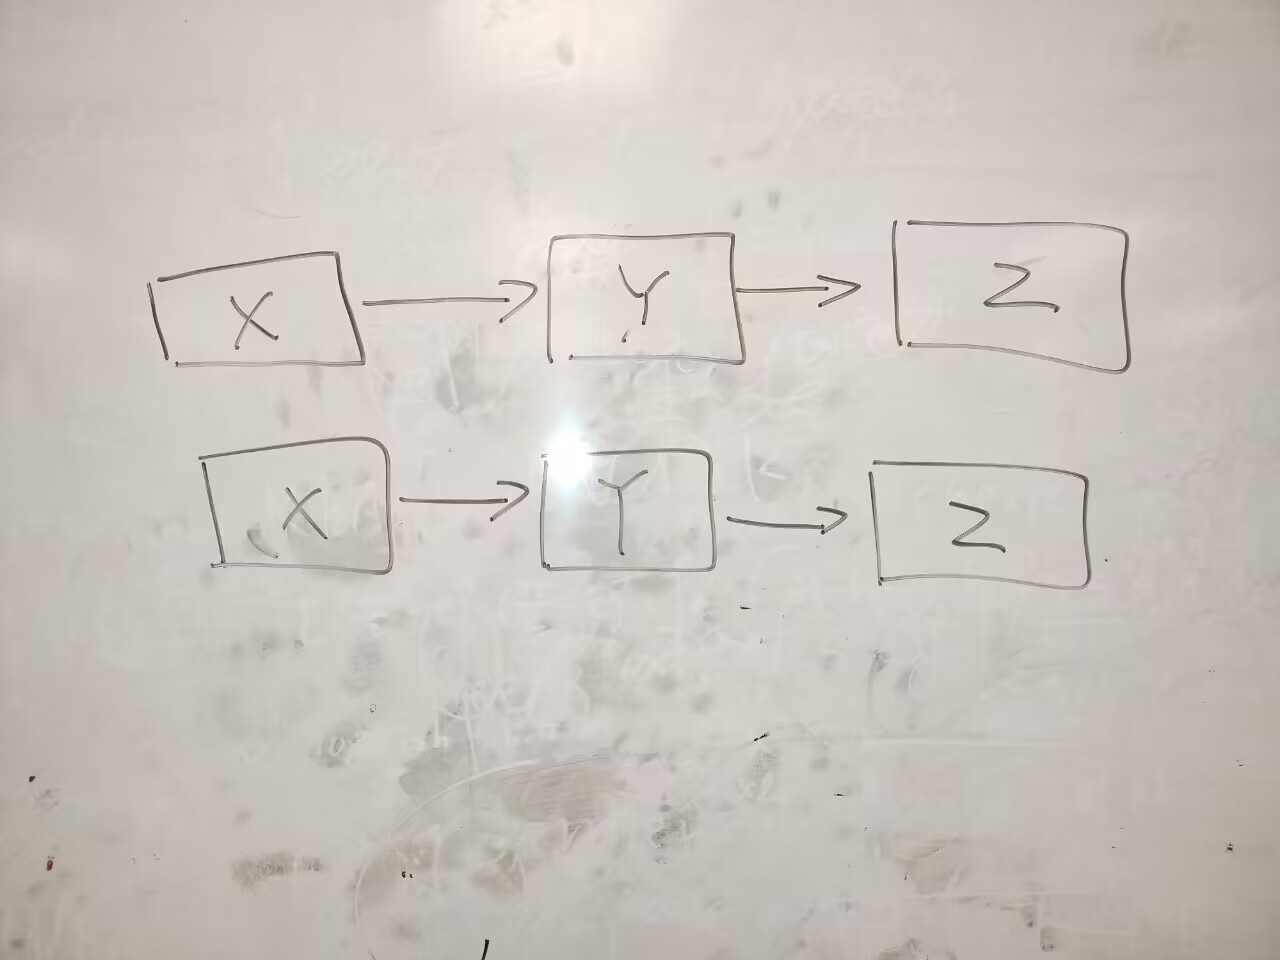
\includegraphics[width=0.5\columnwidth]{img0}
\caption{
  Because the CEK machine is linear and deterministic,
    it can be ``rewound'' to a prior program point
    and be guaranteed to perform exactly the same sequence of states
    as during its prior execution.
  }
\label{fig:replayability}
\end{figure}

One key property guaranteed by determinism is that, for a given
initial program $C$, the machine state at any point during $C$'s
execution can be uniquely identified by how many steps have been
executed since the initial state. In other words, the initial state is
identified with the number $0$, the next state it transitions to with
the number $1$, and so on. Formally, this can be done by extending the
state with a tock and extending every transition $S_1 \to S_2$ with an
increment $t, S_1 \to t + 1, S_2$. This state number, which we call a
``tock'', is logically unbounded, but in our implementation, it is
stored as a 64-bit integer. In our implementation, that suffices for
several decades of runtime on current hardware.

\subsection{Heap Memory}

Because we are interested in
  the memory usage of $\lambda_Z$ program,
  we now extend the CEK machine with an explicit heap
  and explicit pointers.
Values $V$ are now implemented as pointers
  $P\langle \VCell \rangle$ to ``value cells'',
  which can be closures, products, and sums
  and which in turn contain values, that is, pointers.
Kontinuations $K$ are likewise replaced
  with pointers $P\langle \KCell \rangle$
  to ``continuation cells''.
The CEK machine state is now extended
  with a heap $H$;
  we call the extended machine CEK-H.
The heap, pointers, and related methods
  are shown in \Cref{fig:heap};
  the new definitions of values and kontinuations
  are shown in \Cref{adx:cekh}.

\begin{figure}
  \begin{tabular}{\mytableshape}
    Heap & $H$ & $::=$ & An abstract key value store \\
    Pointer to $X$ & $P\langle X \rangle$ & $::=$ & Key into heap with value type $X$ \\
    Lookup & & : & $(P\langle X \rangle, H) \to X$ \\
    Alloc & & : & $(X, H) \to (P\langle X \rangle, H)$ \\
  \end{tabular}
  \caption{The abstract heap / pointer interface for the CEK-H machine.}
  \label{fig:heap}
\end{figure}

CEK transitions now need to
  lookup or store values on the heap
  using the $\Lookup(P, H)$ and $\Alloc(X, H)$ functions.
For example, evaluating a function application $F(X)$
  now requires allocating a $\KApp_0$ cell:
\begin{mathpar}
  \inferrule{\Alloc(\KApp_0~K~X, H) = (P, H')}{\Eval(F(X), \Env, K), H \leadsto \Eval(F, P), H'}
\end{mathpar}
Meanwhile, applying a $\KApp_0$ kontinuation
  requires dereferencing the value pointer
  and then allocating the $\KApp_1$ kontinuation:
\begin{mathpar}
  \inferrule{
    \Lookup(V, H) = \Clos~\Env'~N~C \and
    \Alloc(\KApp_1~\Env'~N~C~K, H) = (P', H')
  }{
    \Apply(\KApp_0~\Env~X~K, V), H \leadsto
    \Eval(X, \Env, P'), H'
  }
\end{mathpar}
The full $\Eval$ and $\Apply$ transition relation
  is given in \Cref{adx:cekh}.

Importantly, every CEK machine step
  (whether $\Eval$ or $\Apply$)
  makes at most one call to $\Lookup$
  and at most one call to $\Alloc$. 
This means that each allocation the program makes
  can be uniquely identified by the tock for the machine state
  when it is allocated.
This identification is the core abstraction that drives \name.
